% METODOLOGIA
\label{chapter:metodo}
Este Capítulo descreve o método proposto neste trabalho , baseado em LLVM, para aprimoramento do método Map2Check para geração de casos de teste de gerenciamento de memória de programas em C.

\section{Método Map2check LLVM}

%\textcolor{red}{}
A \autoref{fig:fluxo_map2check}\footnote{Ícones dos vetores obtidos de \url{br.freepik.com}} demonstra o fluxo do método proposto que consiste em: 
(a) Receber como entrada o código fonte de um programa escrito em C; 
(b) Converter o programa em C para um representação intermediária, neste caso LLVM IR \cite{Lattner:2004}; 
(c) Aplicação de otimizações de código que não removam informações úteis para geração de um contra-exemplo, por exemplo, remoção de código morto \cite{Lattner:2004}; 
(d) Instrumentação do código analisado com funções para o rastreamento de ponteiros (endereços de memória), assertivas e funções para execução simbólica com o \textit{framework} Klee; 
(e) Conexão entre o código instrumentado com uma biblioteca desenvolvida para dar suporte a execução das funções instrumentadas; 
(f) Otimizações no código após a instrumentação do código analisado; 
(g) Execução simbólica do código analisado instrumentado em LLVM IR utilizando o Klee para geração de dados entradas para as funções instrumentadas e validação das assertivas com as propriedades de segurança; e 
(h) Geração de um \textit{log} de rastreamento (\textit{witness}) caso uma propriedade seja violada, ou seja, uma assertiva falhe durante a verificação do código analisado. 
%Durante a fase de instrumentação, são analisadas as seguintes situações: (a) Verifica-se o %tipo de instrução; e (b) Instrumenta-se um método com base no contexto da instrução.

\begin{figure}[htb]
	\caption{\label{fig:fluxo_map2check} Método Map2Check}
	\begin{center}
	    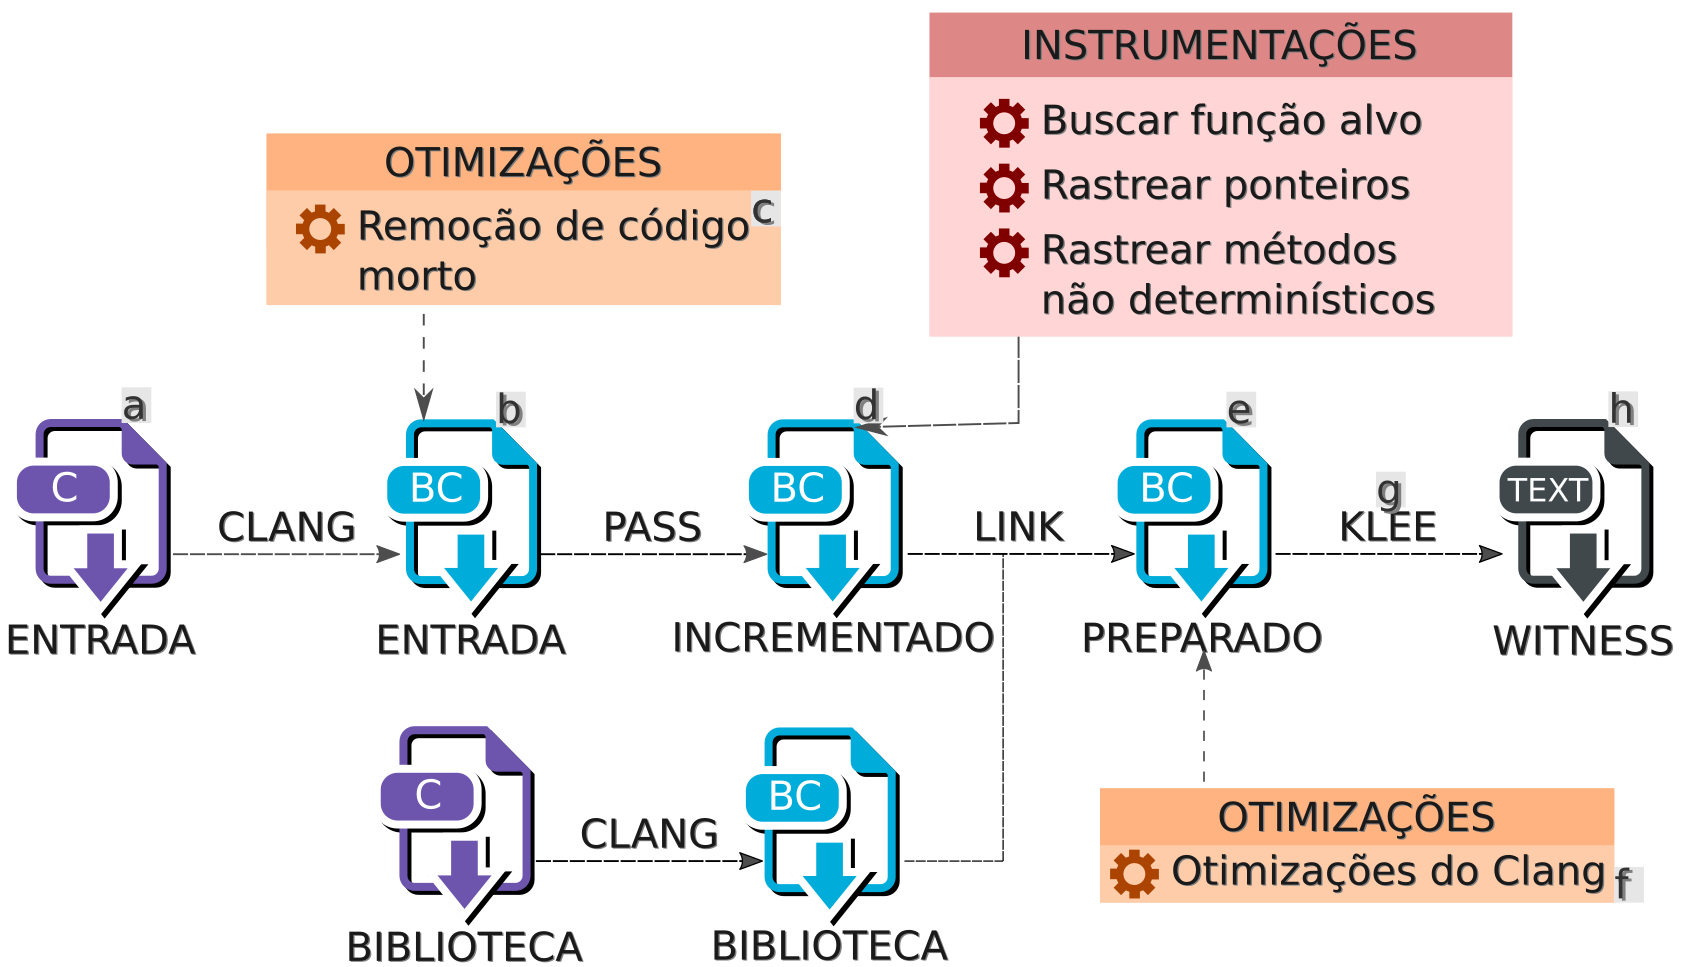
\includegraphics[scale=0.35]{resources/fluxo_map2check.png}
	\end{center}
	\legend{Fonte: Própria}
\end{figure}

A \autoref{fig:invalid_free} contém um exemplo de um programa que contém uma desalocação inválida (\textit{invalid free}), as linhas \texttt{5} e \texttt{6} mostram a alocação de dois ponteiros não inicializados \texttt{A} e \texttt{B}, e nas linhas \texttt{15} e \texttt{16} são desalocados os endereços para onde \texttt{A} e \texttt{B} apontam. Logo, analisando a linha \texttt{12}, onde \texttt{B} recebe o valor de \texttt{A}, quando isso ocorrer o valor prévio de \texttt{B} é perdido, o que irá gerar um erro de desalocação e um vazamento de memória. A função \texttt{non\_det\_int} retorna um valor não-determinístico, ou seja, um valor que o programador só saberá durante a execução, a função \texttt{non\_det\_int} pode retornar qualquer valor arbitrário do tipo \texttt{int}. Na linha \texttt{11}, temos uma condição de decisão no fluxo de execução do código, onde caso o valor de uma variável seja maior do que catorze teremos uma referência perdida, resultado na violação de uma propriedade memória.
%, mas o valor dessa variável depende de outra variável que depende de uma função %não-determínistica, 
O exemplo apresentado na \autoref{fig:invalid_free} demonstra como isso pode ser um problema em um sistema muito complexo, pois podem haver mais camadas de não determinismo ocultas e múltiplas condições problemáticas, tais como: laços aninhados e em programas como \textit{threads} múltiplas trocas de contexto.  

\begin{figure}[thp]
\caption{\label{fig:invalid_free} Programa com desalocação inválida}
\begin{center}
\begin{minipage}{0.8\textwidth}
\begin{lstlisting}[language=C]       
#include <stdio.h>
#include <stdlib.h>

int main(){

  int *A = malloc(10);
  int *B = malloc(10); 
  int x = non_det_int();
  int y = x * 7 - 15;
  
  if(y > 14){
    B = A;           
  }
  
  free(A);  
  free(B);            

  return 0;
}	
\end{lstlisting}
\end{minipage}
\end{center}
\legend{Fonte: Própria}
\end{figure}


Nesta primeira etapa deste TCC, a nova versão do Map2Check não estará utilizando um \textit{model checker} para inferir as propriedades de segurança. O protótipo já desenvolvido utiliza execução simbólica para percorrer o espaço de estados do programa e inferi propriedades para verificação baseadas em chamadas de funções (exemplo, \texttt{ free()}), através de instrumentação do código. A nova versão do Map2Check está disponível em: \url{https://github.com/hbgit/Map2Check/tree/map2checkllvm} 
\par
As propriedades já suportadas pelo novo Map2Check consistem em: erros de desalocação inválida e de alcançabilidade de funções, além de gerar um rastreamento do erro reportado, contendo as informações necessárias sobre como o erro aconteceu.  Esse rastreamento de memória guia os desenvolvedores diretamente para os locais onde os erros de gerenciamento de memória são identificados. 


% -----------------------------------------------------------------
% => Geração da representação intermediária
% -----------------------------------------------------------------
\subsection{Geração de representação intermediária de código}
Para geração do código intermediário (para LLVM-IR)  a partir de um código em C utiliza-se o compilador CLANG com \textit{front-end} para o Map2Check. Assim,  utilizamos o CLANG com as seguintes opções \texttt{-O0 -c -emit-llvm -g}, que significam respectivamente: (a) Não otimizar o código; (b) Não \textit{linkar} com outras bibliotecas; (c) Gerar o LLVM IR; e (d) Adicionar informações de \textit{debug}. Desta forma, a IR do código gerado tem os dados necessários (exemplo, referência ao número da linha do código analisado) para aplicar as análises de forma abrangente e com uma corretude maior.

\newpage
\par
Finalizado a geração do código intermediário, o método aplica otimizações na IR (usando o \textit{framework} LLVM), tais como, a remoção de código morto, ou seja, remoção de todas as partes do código inalcançáveis. Assim, o método elimina partes de código que seria desperdiçada na verificação das propriedades, pois o código nunca seria executado, diminuindo o tempo de execução necessário de execução do método. Após isso, o código intermediário está pronto para ser analisado e instrumentado. A \autoref{fig:vanilla_cfg} mostra o grafo de controle de fluxo (CFG) do código analisado da \autoref{fig:invalid_free} em LLVM IR.

\begin{figure}[H]
	\caption{\label{fig:vanilla_cfg} CFG do programa original}
	\begin{center}
	    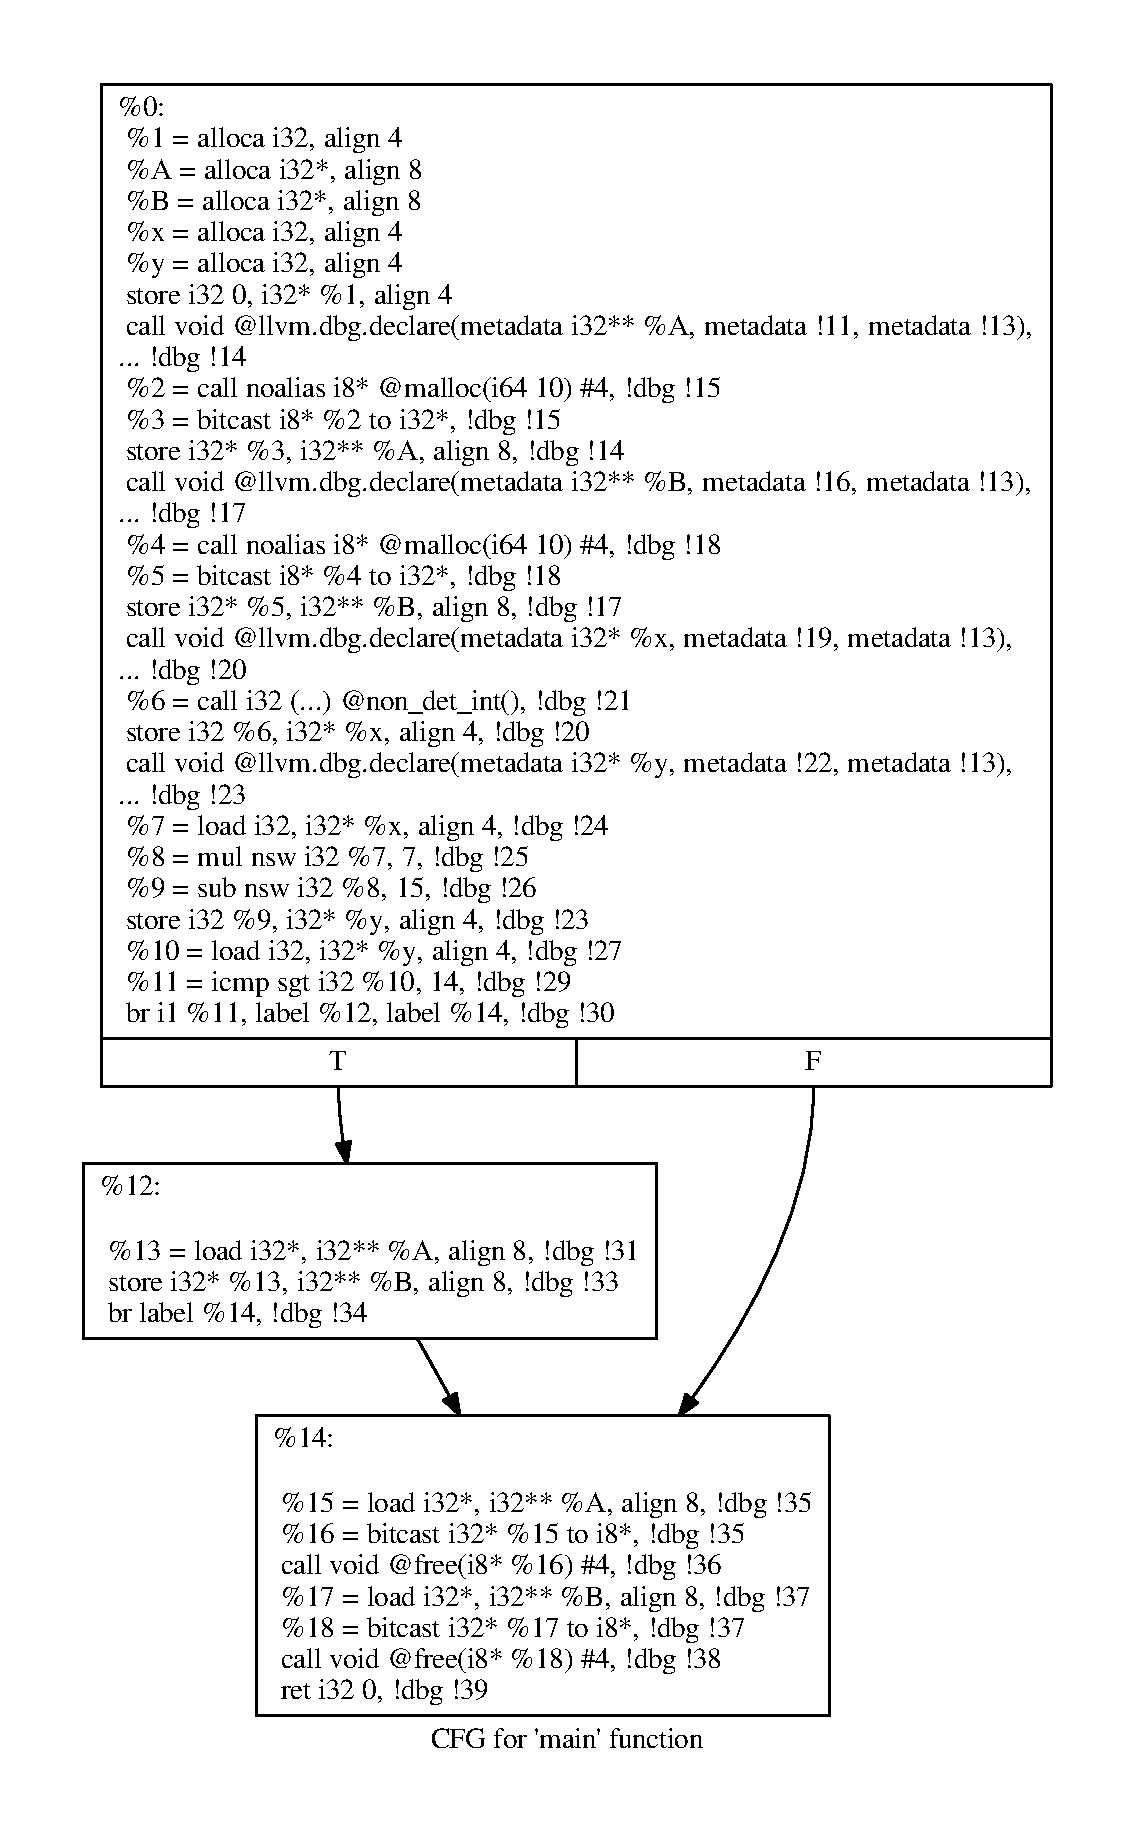
\includegraphics[scale=0.6]{resources/vanilla_cfg.pdf}
	\end{center}
	\legend{Fonte: Própria}
\end{figure}

O programa do CFG da \autoref{fig:vanilla_cfg}, exibe um código em LLVM na versão $3$.$8$.$1$, o código LLVM IR contém diversos comando e operadores, em especial devemos nos atentar as seguintes estruturas:
  \begin{description}
  \item[\textbf{Variáveis:}] Variáveis podem ser nomeadas ou não, caso não tenham nome, um número será utilizado para a representar. Se uma variável nomeada aparecer novamente em outro escopo (porém diferente) o nome será modificado automaticamente (a \autoref{fig:progSameName} mostra um exemplo disso). Exemplos de variáveis seriam \texttt{\%1} e \texttt{\%x}.
  %
  \item[\textbf{Atribuições:}] As instruções com operador \texttt{store} representam atribuições, onde o primeiro argumento é o valor a ser atribuído e o segundo argumento é a variável com endereço de destino. Essas instruções são importantes para realizarmos o rastreio da memória pois se o segundo argumento for um ponteiro (a API do LLVM nos permite diferenciar diretamente) significa que devemos acompanhar seus valores. 
%  
  \item[\textbf{Chamadas de função:}] O operador \texttt{call} define chamadas de funções, esse operador é útil para nossa análise por ser um jeito simples de rastreio dos métodos de diferentes linguagens (desde seja adicionado o suporte).
  %
  \item[\textbf{Metadados:}] Os metadados contém informações úteis referentes a instrução atual antes da compilação, por exemplo, número da linha e escopo. Essas informações são úteis para geração do contra-exemplo. 
  %
\end{description}

\begin{figure}[htb]
\caption{\label{fig:progSameName} Exemplo de programa com variável com mesmo nome em escopos diferentes}
\begin{center}
\begin{minipage}{0.5\textwidth}
\begin{lstlisting}[language=C]       
int x;
{
    int x;
}  
\end{lstlisting}
\end{minipage}
\end{center}
\legend{Fonte: Própria}
\end{figure}
% -----------------------------------------------------------------
% => Transformação de código
% -----------------------------------------------------------------
\subsection{Transformação de código}

%Essa subseção irá tratar sobre como são feitas 
As transformações no código analisado ocorrem na representação intermediário gerado pelo método, no formato LLVM IR (seguindo o padrão em \textit{Static Single Assignment} (SSA)). 
As transformações aplicadas consistem em adicionar funções da biblioteca da \autoref{sub:biblioteca} \textbf{biblioteca para rastreamento de memória e assertivas}, sendo que os 
argumentos para as funções e assertivas são obtidos analisando as instruções no código intermediário.
%são instrumentados e seus argumentos obtidos

\par
%Após a geração da 
A representação intermediária do código analisado é lido 
%, é feito uma análise em cima dela, e com base 
para identificar cada tipo de instrução como declarações, atribuições e chamadas de funções 
para executar um instrumentação de código baseada em funções suportadas por uma biblioteca do método proposto. 
%na instrução atual é adicionado uma chamada com o método adequado. 
Essas instrumentações tem os seguintes objetivos: 
(a) Buscar uma função alvo, ou seja, uma chamada de uma função especifica ou mesmo uma localização de erro no código; 
(b) Rastrear operações sobre ponteiros; 
(c) Rastrear funções não determinísticas; e 
(d) Liberar todos os recursos alocados para a validação. 
A \autoref{fig:cfg_pass} exibe o CFG do programa da \autoref{fig:invalid_free} após a instrumentação.


\begin{figure}[H]
	\caption{\label{fig:cfg_pass} CFG do programa após instrumentação}
	\begin{center}
	    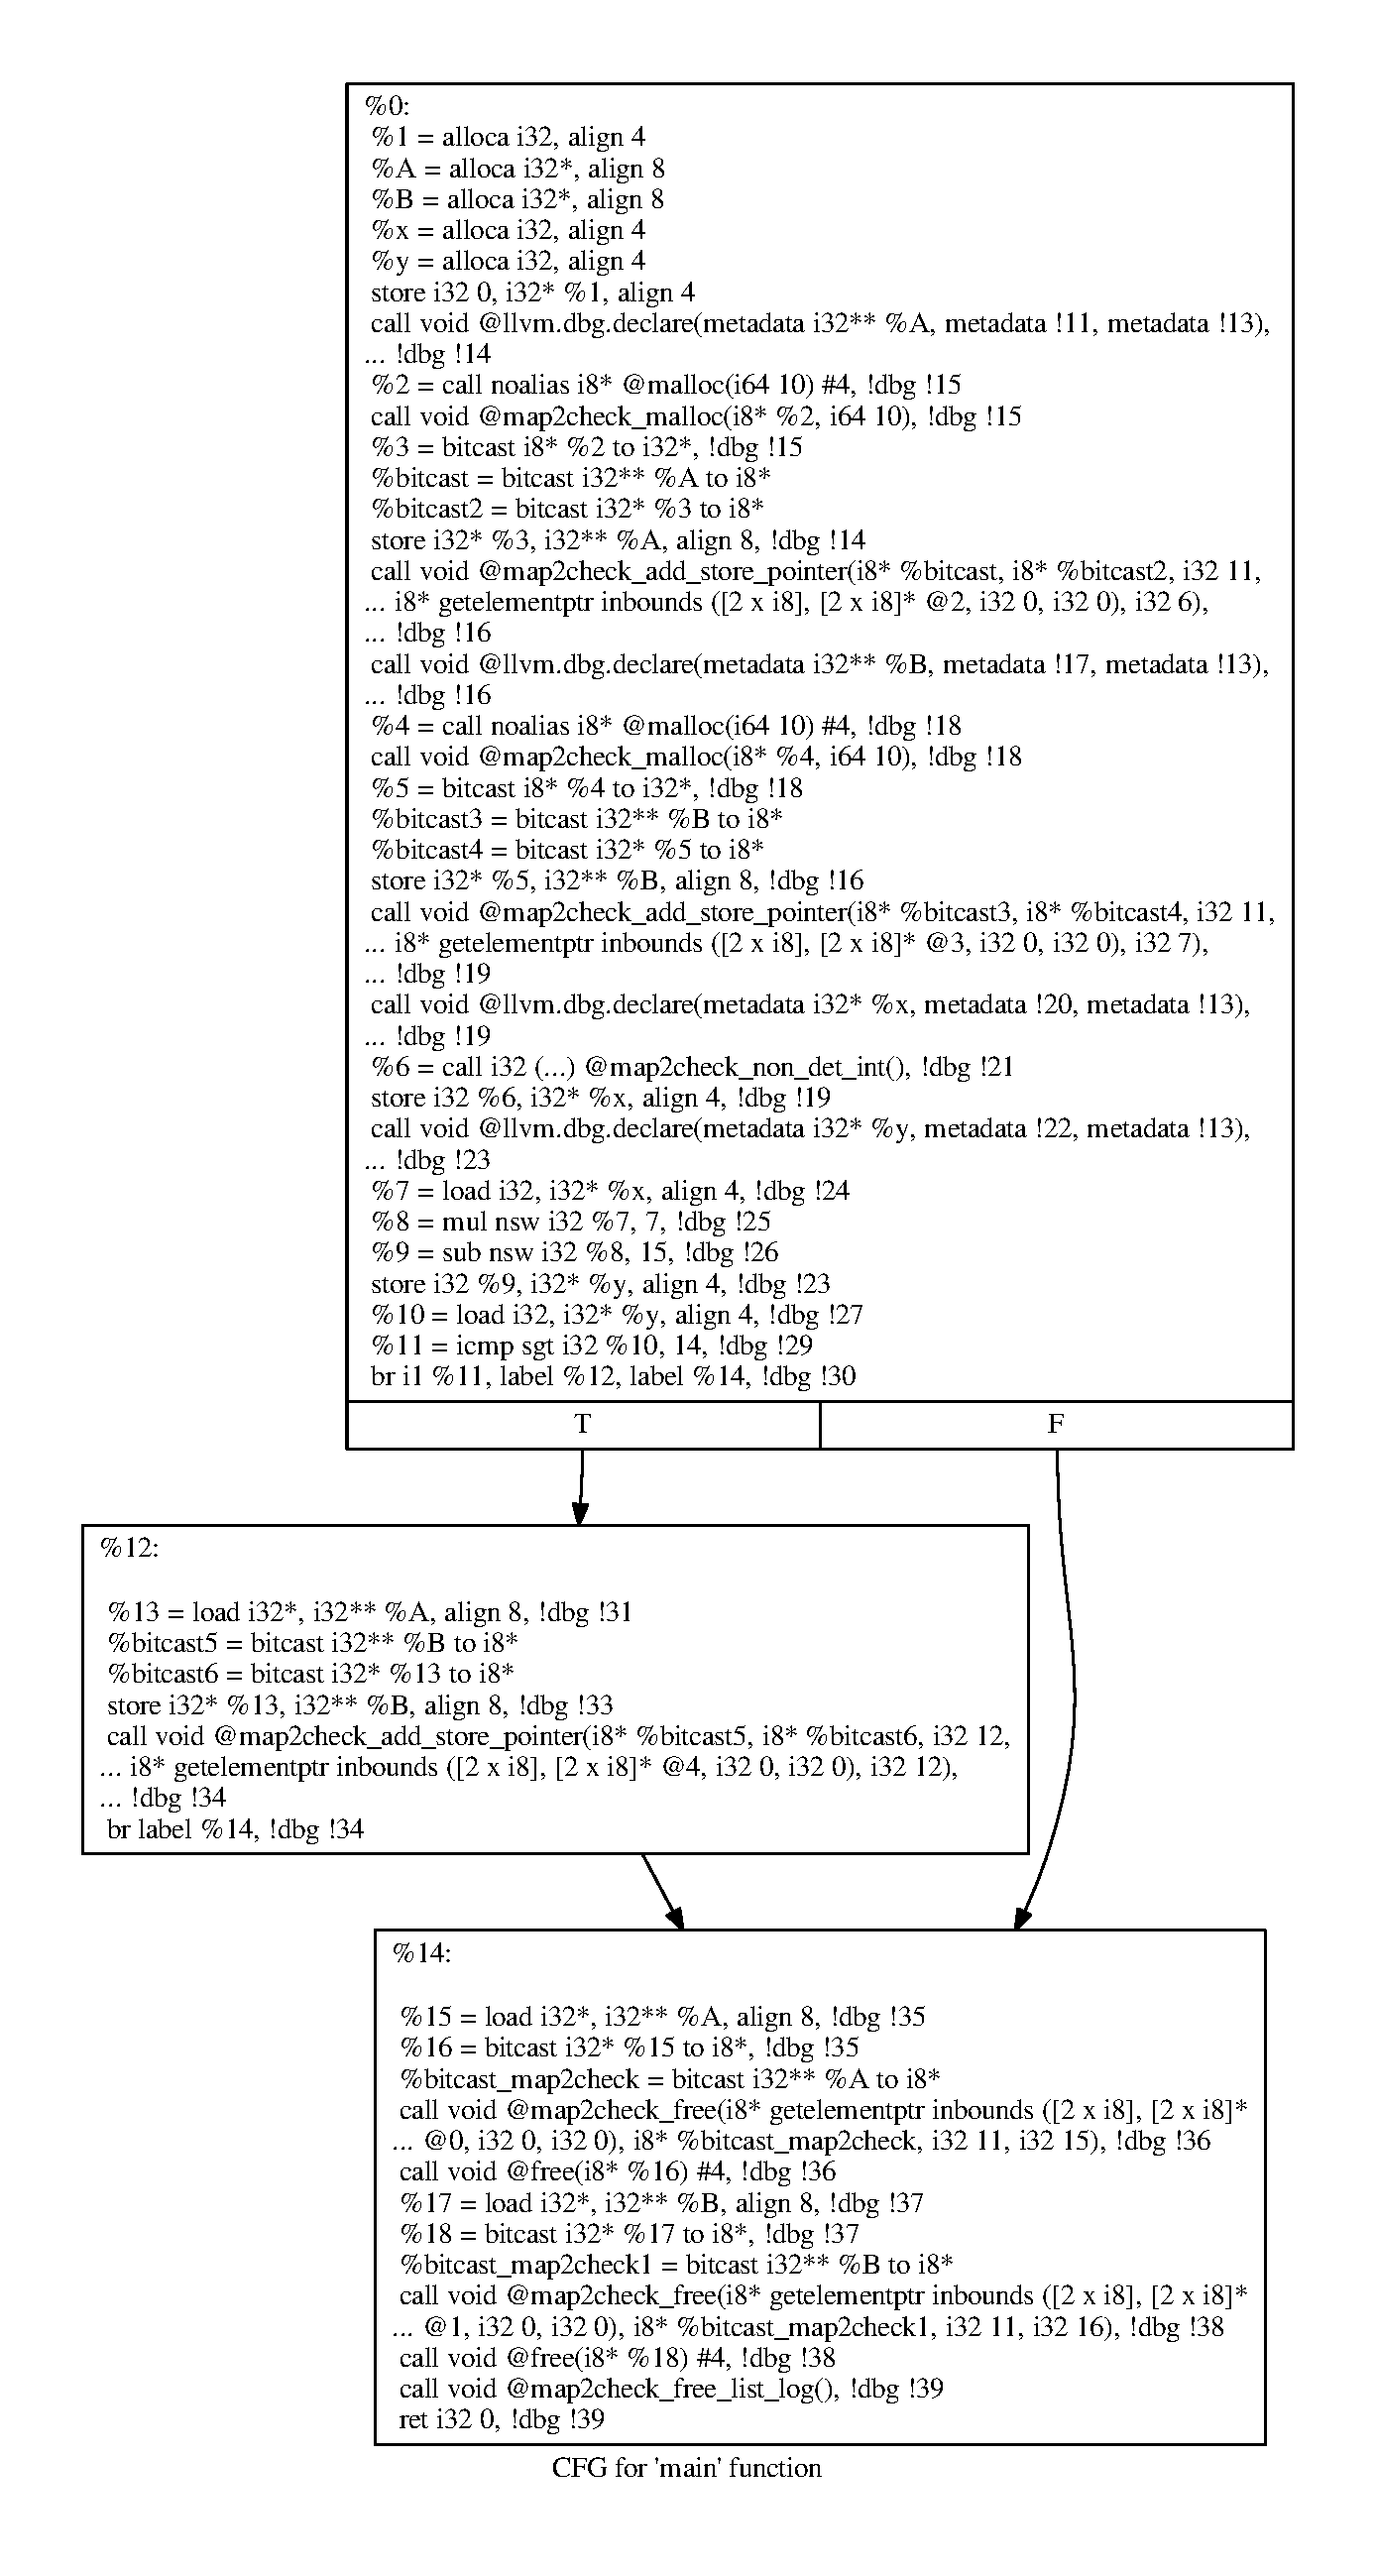
\includegraphics[scale=0.45]{resources/cfg_pass.pdf}
	\end{center}
	\legend{Fonte: Própria}
\end{figure}

Visando automatizar a instrumentação de código é utilizado o seguinte 
%Para obter isso foi utilizado um 
algoritmo, a \autoref{fig:algoritmo_instrumentacao} exibe o algoritmo utilizado para a instrumentação. Como um dos objetivos do LLVM é ser uma suíte para análises e transformações de código\cite{Lattner:2004}, ele dispõe de \textit{pass} que é uma forma modularizada de implementar as análises ou transformações em um código LLVM IR, não precisando ser integrado ao LLVM, pois basta compilar o \textit{pass} separadamente. Para a implantação do algoritmo foram utilizados três \textit{FunctionPass} onde o algoritmo é executado em cada função do programa. O algoritmo consiste em checar todas as instruções de todos os blocos básicos, então analisa a instrução e baseado na análise, instrumenta 
%o método adequado. 
a função de rastreamento ou assertiva com a sua respectiva propriedade de segurança. 

A complexidade do tempo de execução do algoritmo, na \autoref{fig:algoritmo_instrumentacao} é $O(n \times m)$ onde $n$ é o número de instruções do código intermediário e $m$ é a quantidade total de funções do programa analisado a ser comparada com uma função alvo a ser rastreada.
% e $o$ é a quantidade de operações sobre a memória e ponteiros.}
%A complexidade do tempo de execução do algoritmo, na \autoref{fig:algoritmo_instrumentacao}, é $O(n \times m)$ onde $n$ é o número de instruções do código intermediário e $m$ e o quantidade de operações sobre a memória e ponteiros. 

\begin{figure}[H]
	\caption{\label{fig:algoritmo_instrumentacao} Algoritmo utilizado para instrumentação}
	\begin{center}
\begin{algorithmic}[1] 
        \Function{Instrumentação}{Função} \Comment O($n \times m$)
            \ForAll{Instrução $\in$ Função} \Comment O($n$) 
                    \Switch{Instrução.tipo} %\Comment O($m$)
                    	\Case{CallInst} 
                        	\State i $\gets$ (CallInst) Instrução
                            \If{i.funcao.nome $\in$ ListaFunçõesAlvo} \Comment O($m$)
                            	\State InstrumentarFunçãoAlvo() 
                            \EndIf                           
                            \Switch{i.funcao.nome}
                            \Case{matchRegex("\_\_VERIFIER\_NONDET\_")}
                               \State InstrumentarKlee() 
                            \EndCase
                            \Case{"free"}
                                \State InstrumentarDesalocação() 
                            \EndCase
                                \Case{"malloc"}
                                    \State InstrumentarAlocação()
                                \EndCase                                
                            \EndSwitch
                        \EndCase
                        \Case{StoreInst}  
                        	\State i $\gets$ (StoreInst) Instrução
                        	\If{i.operando.tipo = Ponteiro}
                            	\State InstrumentarOperacaoPonteiro()  
                            \EndIf
                        \EndCase
                    \EndSwitch
                 \EndFor                            
            \If{Função.nome = "main"}            	
            	\State InstrumentarLiberaracaoRecursos() 
            \EndIf
        \EndFunction
\end{algorithmic}
	\end{center}
	\legend{Fonte: Própria}
\end{figure}


% -----------------------------------------------------------------
% => Biblioteca para rastreamento de memória e assertivas
% -----------------------------------------------------------------
\subsection{Biblioteca para rastreamento de memória e assertivas}
\label{sub:biblioteca}

Visando prover suporte a verificação das propriedades abordadas pelo Map2Check que utiliza instrumentação de funções foi necessário implementar uma biblioteca com as seguintes capacidades: 
(a) Criar um rastreamento das operações de ponteiros; 
(b) Execução de assertivas baseada em operações com listas; 
(c) Criar rastreamento das operações dinâmicas da memória, alocação e desalocação; 
(d) Gerar informações de \textit{debug}; e 
(e) Manter o fluxo original do programa inalterado.

\par
A biblioteca do método Map2Check é escrita em C, e somente então compilada para LLVM IR, por C ser uma linguagem de alto nível isso trás vantagens durante o processo de desenvolvimento, como manutenabilidade e modularização. Logo, após a compilação da biblioteca de C para LLVM IR é feito o processo de linkedição com o código analisado ser instrumentado. A \autoref{fig:progHeaderFunctions} exibe as funções que podem ser instrumentadas.

\begin{figure}[htb]
\caption{\label{fig:progHeaderFunctions} Funções utilizadas para instrumentação}
\begin{center}

\begin{lstlisting}[language=C]    
//Função para liberar recursos alocados 
void map2check_free_list_log(); 

// Função para debug, imprime o LIST LOG
void map2check_list_debug(); 

// Gera um inteiro não determinístico
int map2check_non_det_int(); 

// Função para acompanhar valores alocados
void map2check_malloc(void* ptr, // Endereço alocado
                      int size); // Tamanho em bytes do endereço

// Função para gerar erro em funções alvo caso seja alcançado           
void map2check_target_function(const char* func_name, // Nome da função
                               int scope, // Escopo onde foi alcançada
                               int line); // Linha onde foi alcançada

/* Função para acompanhar valores desalocados e gerar erros
 * (caso necessário) */                         
void map2check_free(const char* name,  /* Nome da variável passada como 
                                        * argumento (pode ser uma string 
                                        * vazia) */
                    void* ptr,      // Endereço a ser desalocado
                    unsigned scope, // Escopo da chamada do free
                    unsigned line,  // Linha da chamada do free
                    const char* function_name); /* Nome da função onde
                                                 * o free foi chamado */

/* Função para companhar todas as atribuições que variáveis 
 * do tipo ponteiro sofrem */                   
void map2check_add_store_pointer(void* var,   // Endereço da variável
                                 void* value, /* Endereço para onde 
                                               * a variável aponta */
                                 unsigned scope,   // Escopo da atribuição
                                 const char* name, // Nome da variável
                                 int line);        // Linha da atribuição
\end{lstlisting}
\end{center}
\legend{Fonte: Própria}
\end{figure}


% -----------------------------------------------------------------
% => Rastreamento de memória
% -----------------------------------------------------------------
\subsubsection{Rastreamento de memória}

O rastreamento de memória tem como objetivo a verificação da segurança de ponteiros, a identificação de ponteiros nos permite analisar: desalocações inválidas, ponteiros inválidos e vazamentos de memória. Este rastreamento consiste em criar uma lista com atributos sobre as operações de ponteiros para identificar: 
(a) alocações de memória; 
(b) desalocações de memória; e 
(c) operações de atribuições sobre ponteiros. 

\begin{figure}[htb]
	\caption{\label{fig:tabela} Exemplo de LIST\_LOG}
	\begin{center}
	    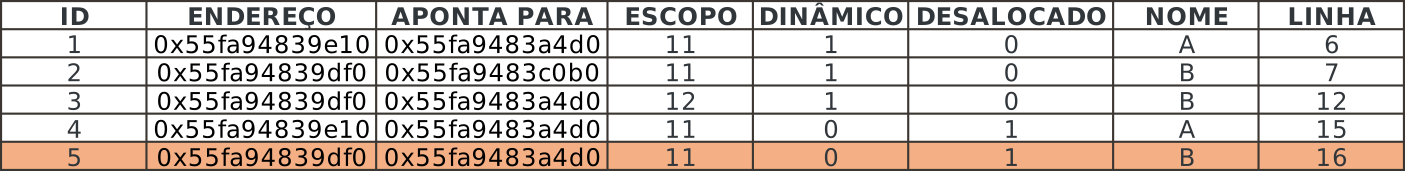
\includegraphics[scale=0.4]{resources/tabela_list_log.png}
	\end{center}
	\legend{Fonte: Própria}
\end{figure}

As informações do rastreamento são armazenadas em uma estrutura chamada LIST\_LOG, contendo informações como: 
nome de variável; 
endereço de memória; 
endereço de memória para onde um ponteiro aponta; 
escopo da variável analisada; 
se o endereço de memória apontado é dinâmico; 
se o endereço de memória está sendo liberado; e 
o número da linha nó código da variável analisado. 
A \autoref{fig:tabela} exemplifica como essa estrutura se comportaria durante a verificação do programa da \autoref{fig:invalid_free} com $y > 14$. 
Analisando os dados do rastreamento gerado na \autoref{fig:tabela} podemos verificar: 
(a) o endereço de memória que foi perdido (ID $2$); e 
(b) a desalocação em de memória do ponteiro \texttt{B} será inválida.

% -----------------------------------------------------------------
% => Rastreio de funções não determinísticas
% -----------------------------------------------------------------
\subsubsection{Rastreio de funções não determinísticas}

O rastreio de funções não determinísticas (funções que retornam um valor que pode variar durante a execução do programa) ocorre ao verificar se a instrução é uma chamada de um método não determinístico previamente definido que retorna um valor arbitrário de um tipo indicado \cite{beyer:2016}. Identificada a função não determinística partir é feito uma instrumentação de uma função para o Klee que irá gerar um valor baseado em execuções simbólicas.
\par
A instrumentação de função para o Klee consiste em criar uma nova variável no programa analisado com o tipo igual ao tipo do não-determinismo identificado (instrumenta-se um inteiro caso seja pedido um inteiro não-determinístico), dessa forma é solucionado um dos possíveis problemas que seria a chamada de um método com um valor não determinístico (apenas com utilização de variáveis temporárias) como: \texttt{if(non\_det\_int())}, durante a execução de código o valor de dentro do \texttt{if} será armazenado em uma variável temporária. A \autoref{fig:progNonDet} exibe um programa com uma chamada de método não-determinístico e a \autoref{fig:progNonDetKlee} mostra como ficaria após instrumentado,   a \autoref{fig:progNonDetInt} exibe a implementação do método.

\begin{figure}[H]
\caption{\label{fig:progNonDet} Programa com método não-determinístico}
\begin{center}
\begin{minipage}{0.8\textwidth}
  \begin{lstlisting}[language=C]
int main() {
  if (non_det_int()) {
    return 1;
  }
  return 0;
}
\end{lstlisting}
\end{minipage}
\end{center}
\legend{Fonte: Própria}
\end{figure}

\begin{figure}[H]
\caption{\label{fig:progNonDetKlee} Programa instrumentado com Klee}
\begin{center}
\begin{minipage}{0.8\textwidth}
  \begin{lstlisting}[language=C]
int main() {
  if (map2check_non_det_int()) {
    return 1;
  }
  return 0;
}
\end{lstlisting}
\end{minipage}
\end{center}
\legend{Fonte: Própria}
\end{figure}


\begin{figure}[H]
\caption{\label{fig:progNonDetInt} Implementação do método que instrumenta o Klee}
\begin{center}
\begin{minipage}{0.8\textwidth}
  \begin{lstlisting}[language=C]
int map2check_non_det_int() {
  int non_det;
  klee_make_symbolic(&non_det,
                     sizeof(non_det),
                     "non_det_int");
  return non_det;
}
\end{lstlisting}
\end{minipage}
\end{center}
\legend{Fonte: Própria}
\end{figure}

% -----------------------------------------------------------------
% => Rastreio de funções alvo
% -----------------------------------------------------------------
\subsubsection{Rastreio de funções alvo}

Segundo \citeonline{beyer:2016} apartir de um conjunto de estados iniciais de um programa na chamada da função \texttt{main}. A definição $ LTL(f) $ especifica que a fórmula $f$ é verdadeira para cada um dos estados iniciais. Assim, a fase de instrumentação consiste em localizar a função alvo e logo antes dela, adicionar uma função da biblioteca, assim verificando se ao longo da execução essa função foi chamada.

\par
Para exemplificar isso temos a \autoref{fig:progExampleTarget} onde temos a função não determinística \texttt{non\_det\_int()} e a função alvo \texttt{TARGET()}, observemos que: (a) a linha 2 contém uma chamada não determinística; e (b) a função alvo se encontra na linha 4. A \autoref{fig:progExampleTargetInstrumented} exemplifica a instrumentação, nesse exemplo, é assumido que o escopo é 1, esse escopo normalmente é determinado durante a compilação. O método instrumentado \texttt{map2check\_target\_function} ao ser executado, demostra que a localização seria alcançada, injetando uma assertiva de erro na localização onde ocorre a chamada da função alvo.

\begin{figure}[H]
  \caption{\label{fig:progExampleTarget} Exemplo de função alvo}
  \begin{center}
    \begin{minipage}{0.8\textwidth}
      \begin{lstlisting}[language=C]
int main() {
    int x = non_det_int();
    if (x > 10) {
      TARGET();
    }
}
\end{lstlisting}
\end{minipage}
\end{center}
\legend{Fonte: Própria}
\end{figure}

\begin{figure}[H]
\caption{\label{fig:progExampleTargetInstrumented} Exemplo de função alvo após instrumentação (assumindo escopo 1)}
\begin{center}
\begin{minipage}{0.8\textwidth}
  \begin{lstlisting}[language=C]
int main() {
    int x =  map2check_non_det_int();
    if (x > 10) {
      map2check_target_function("main", 1, 4);
      TARGET();
    }
}
\end{lstlisting}
\end{minipage}
\end{center}
\legend{Fonte: Própria}
\end{figure}


% -----------------------------------------------------------------
% => Verificação das propriedades de segurança
% -----------------------------------------------------------------
\subsection{Verificação das propriedades de segurança}

A verificação do programa analisado consiste em determinar se 
%Para gerar o resultado sobre um 
o programa analisado satisfaz ou viola suar propriedades de segurança, no caso do Map2Check
as assertivas instrumentadas. Assim, caso uma propriedade seja violada então é gerado uma contraexemplo contendo o rastreamento de acesso aos endereços de memória. 
Neste trabalho, já esta sendo projetado que o Map2Check gere uma 
%, faz-se uso de uma ou mais textit{witness} (testemunha) para o testemunho. 
%Testemunho é o processo onde cada 
\textit{witness}/evidências (\cite{beyerA:2015}) que apresente evidências sobre a violação ou não das propriedades de segurança. Segundo \cite{beyerA:2015}, as ferramentas de verificação são responsáveis por gerar as evidências sobre o resultado da verificação de propriedades, onde tais evidências puderam ser utilizadas por ferramentas de \textit{witness checker} (como o Ultimate Automatizer \cite{Heizmann:2015} e CPAChecker \cite{Beyer:2011}) que irão validar o resultado gerado por um verificador. 
\par
Neste momento do trabalho o \textit{witness} ainda não é gerado automaticamente, porém, já podemos obter informações relevantes para a geração das evidências. Ao Klee ser executado, podemos analisar quais casos, dados gerados na execução simbólica, podem criar um execução no programa que apresenta a violação de uma propriedade. Por exemplo, analisando a execução do programa da \autoref{fig:invalid_free} obtemos como entrada $ x = 7 $, o que podemos verificar que é um caso onde a propriedade de segurança de desalocação de memória é violada. 
%
Outro exemplo seria a execução do programa da \autoref{fig:targetFunction}, ao executarmos o Map2Check com esse programa e adicionarmos TARGET\_FUNCTION como função alvo (através de \texttt{-f TARGET\_FUNCTION} ao executar), obtemos como entrada $ x = 2 $, onde a a função é alcançada, demonstrado que se a dada localização da função fosse uma localização/estado de erro está poderia ser alcançada.
%propriedade de segurança de alcançabilidade é violada.


\begin{figure}[H]
	\caption{\label{fig:targetFunction} Programa com função alvo}
	\begin{center}
    \begin{lstlisting}[language=C]     
int main(){

  int x = non_det_int();
  int y = x * 9;
  
  if(y > 14){
    TARGET_FUNCTION();
  }
  return 0;
}	
	\end{lstlisting}
	\end{center}
    \legend{Fonte: Própria}
\end{figure}

